\documentclass[10pt,journal,compsoc,UTF8]{IEEEtran}
\usepackage{CTEX}
%%去掉UTF8和\usepackage{CTEX}之后,摘要/附录/参考文献就会变成英文的
\ifCLASSOPTIONcompsoc
  % IEEE Computer Society needs nocompress option
  % requires cite.sty v4.0 or later (November 2003)
  \usepackage[nocompress]{cite}
\else
  % normal IEEE
  \usepackage{cite}
\fi
\usepackage{graphicx,subfigure,color,multirow,amsmath}
\usepackage[super,square,numbers,sort&compress]{natbib} % for super citation
\usepackage{url}
\usepackage{latexsym}
\usepackage{float}
\usepackage{listings}
\usepackage{xcolor}
\usepackage{caption}
\usepackage{amsfonts,amssymb}
\usepackage{framed}
\usepackage{pdfpages}
\lstset{
    numbers=left, 
    numberstyle= \tiny, 
    keywordstyle= \color{ blue!70},
    commentstyle= \color{red!50!green!50!blue!50}, 
    frame=shadowbox, % 阴影效果
    rulesepcolor= \color{ red!20!green!20!blue!20} ,
    escapeinside=``, % 英文分号中可写入中文
    xleftmargin= 2em,
    xrightmargin= 0em, 
    aboveskip=1em,
    framexleftmargin=2em
} 
  
% *** GRAPHICS RELATED PACKAGES ***
%
\ifCLASSINFOpdf
  % \usepackage[pdftex]{graphicx}
  % declare the path(s) where your graphic files are
  % \graphicspath{{../pdf/}{../jpeg/}}
  % and their extensions so you won't have to specify these with
  % every instance of \includegraphics
  % \DeclareGraphicsExtensions{.pdf,.jpeg,.png}
\else
  % or other class option (dvipsone, dvipdf, if not using dvips). graphicx
  % will default to the driver specified in the system graphics.cfg if no
  % driver is specified.
  % \usepackage[dvips]{graphicx}
  % declare the path(s) where your graphic files are
  % \graphicspath{{../eps/}}
  % and their extensions so you won't have to specify these with
  % every instance of \includegraphics
  % \DeclareGraphicsExtensions{.eps}
\fi
\hyphenation{op-tical net-works semi-conduc-tor}

%%文档开始
\begin{document}
%%标题,\\强制断行
\title{Depth from Videos in the Wild:Unsupervised Monocular Depth Learning from Unknown Cameras}

%%作者
\author{Anakin~Skywalker,
        Han~Solo,
        and~R2-D2}


% 页眉
\markboth{Journal of \LaTeX\ Class Files,~Vol.~16, No.~8, October~2018}%
{Shell \MakeLowercase{\textit{et al.}}: Bare Demo of IEEEtran.cls for Computer Society Journals}

\IEEEtitleabstractindextext{%
\begin{abstract}
%%摘要
我们提出了一种新颖的方法,用于同时从单目视频中学习深度、自我运动、对象运动和相机内参,仅使用相邻视频帧之间的一致性作为监督信号。与先前的工作类似,我们的方法也是通过对帧应用可微分的重投影并将结果与​​相邻帧进行比较来学习,但是提供了一些改进:我们直接使用训练期间预测的深度图以几何方式可微地解决遮挡问题。我们引入了随机层归一化,一种新颖的正则化器,并考虑了场景对象的运动。据我们所知,我们的工作是第一个以无监督的方式从视频中学习相机参数(包括镜头畸变)的方法,从而使我们能够从未知来源的任意视频中提取准确的深度和运动。我们在Cityscapes,KITTI和EuRoC MAV数据集上评估了我们的方法,深度预测和里程测量达到先进水平,并定性证明了可以从YouTube视频集合中学习深度预测。该代码是公开可用的。
\end{abstract}


\begin{IEEEkeywords}
  %%关键词
\end{IEEEkeywords}}


% make the title area
\maketitle

\IEEEdisplaynontitleabstractindextext

\IEEEpeerreviewmaketitle
%%Introduction标题
\IEEEraisesectionheading{\section{Introduction}\label{sec:introduction}}

%%Introduction文字(提一个字母加特技)
\IEEEPARstart{M}{achine} learning, 从视频估计3D结构和摄像机运动是计算机视觉中的关键问题。解决此问题的传统方法依赖于在多个连续帧中识别场景中的相同点,然后求解在这些帧之间最大一致性的3D结构和摄像机运动[23]。但是,只能针对所有像素的子集建立帧之间的这种对应关系,这留下了无法确定的深度估计问题。通常根据连续性平面性等假设来填充空隙。
  
深度学习无需从数据中手动指定这些假设。在信息不足以解决歧义的地方,深度网络可以通过从之前看到的例子进行归纳得出深度图和flow felds。无监督方法允许仅从原始视频中学习,使用与传统方法相似的一致性损失,但可以在训练过程中对其进行优化。推论得出,训练有素的网络能够根据单个图像预测深度,并根据成对的或更长的图像序列预测相机运动。

随着在这个方向上的研究获得关注[47,10,12,33,24,34],很明显,物体运动是主要障碍,因为它违反了静态场景的假设。已经提出了解决该问题的几种方法[44,40],包括通过实例分割[6]来利用对场景的语义理解。遮挡是另一个限制因素,最后,在此方向上的所有先前工作中,都必须提供相机的内参。
\begin{figure}[htbp]
  \begin{framed}
      \centering
    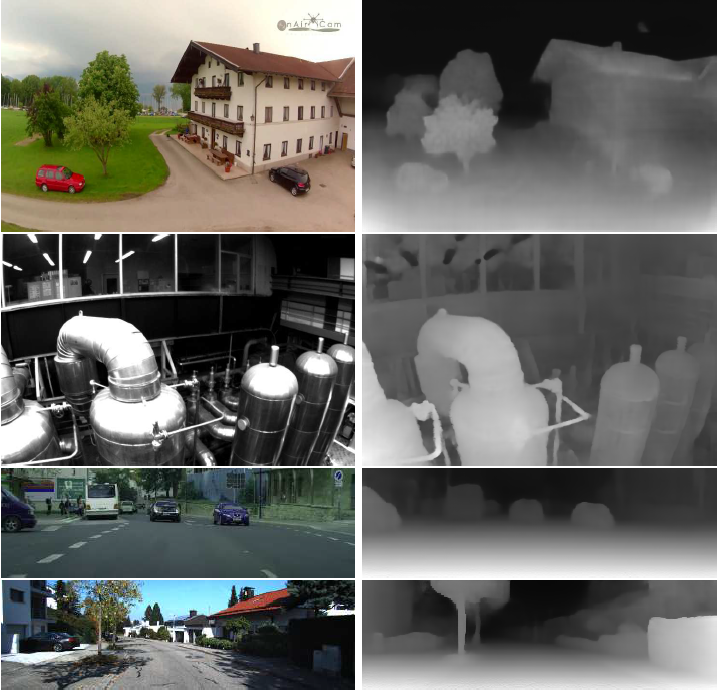
\includegraphics[width=1\linewidth]{imgs/1.png}\\
  \caption{从未知来源的视频中学习到的深度,同时学习相机内外参数由于我们的方法不需要了解相机参数,因此可以将其应用于任何视频集所有深度图(如右图所示,以视差图方式表示)都是从原始视频中预测的数据来源从上到下为:YouTube8M [1],EuRoC MAV数据集[5],Cityscapes [7]和KITTI [11]的。}
  \end{framed}
\end{figure}

这项工作解决了上述问题,因此减少了监督并提高了未标记视频的深度和运动预测的质量。首先,我们证明了可以训练一个深层网络来预测摄像机的内参,包括镜头畸变,并且不受视频本身的影响(见图1)。第二,在这种情况下,我们是第一个以几何方式从预测深度直接解决遮挡问题的方法。最后,我们大大减少了解决场景中移动元素所需的语义理解:代替分割运动对象的每个实例并在帧之间进行跟踪[6],我们需要一个单独的蒙版来覆盖可能属于某个运动物体的像素。此蒙版可以像矩形边界框的并集一样粗糙。与实例分割相比,获得这种粗糙的遮罩要简单得多,并且可以使用现有模型更可靠地解决。
除了这些定性的进步外,我们对我们的方法进行了广泛的定量评估,发现它在多个广泛使用的基准数据集效果显著。将数据集集中在一起可以提高模型质量。最后,我们首次证明了可以在YouTube视频上学习深度和相机内参,这些视频是用多个不同的相机捕获的,每个相机具有未知且通常不同的内参。


\section{Related work}
估计场景深度是机器人导航和操纵的重要任务。历史上已经进行了大量研究,包括有关立体、多视图几何和主动感应的大量研究[29,21,9]。近来,基于学习的密集深度预测方法受到关注[9,22,19,45]。其中,根据输入的RGB图像预测场景深度,并使用由传感器(如LiDAR)提供的监督来学习深度估计功能。类似的方法也可用于其他密集预测,例如表面法线[8,38]。

\subsection{无监督深度学习}
无监督学习深度信息,其中仅从单目视频本身获得监督而无需深度传感器的方法,最近也得到了普及[47、10、12、33、24、34、44]。

Garg等[10]介绍了深度学习和自我运动的联合学习。Zhou等[47]提出了一种完全可微的方法,其中深度和自我运动是由深度神经网络共同预测的。用于单目[33、42、24、41、44、35、6]和双目[12、33、40、46、35、46]的技术。后者表明在训练过程中使用双目输入时,深度图质量得到改善。一些方法可以直接学习视差[17,18,43]。其他新颖的技术包括使用运动[41、35、44、6、40]。

\subsection{使用参数未知的相机}
这是一个活跃的研究领域,专注于单视图或多视图图像[2、30、20]。如Li[20]所示,由于输入源的多样性和缺乏相机参数,对于互联网照片而言尤其困难。我们的工作通过学习相机内参,为解决这一挑战迈出了一步。

\subsection{遮挡感知}
[36、15、25]使用非几何学的方法来处理光流中的遮挡。可微分网格渲染[26,16]对遮挡采用了几何方法。在学习预测深度和相机自我运动的情况下,通过学习可解释性掩码[47],通过惩罚前一帧或下一帧到中间的最小重投影损失以及通过光流来解决[40]。在后一种情况下,我们是第一个通过可微分损失以直接几何方法解决遮挡的方法。

\subsection{内参的深度学习}
学习预测相机的内参主要限于严格监督的方法。GT的来源各不相同:Workman等[37]使用从运动中采用经典一维结构估算的焦距作为GT。Yan等人[39]基于EXIF获得焦距。Bogdan等人[4]使用具有已知内参(包括失真)的虚拟相机从全景图合成相片。据我们所知,我们的方法是唯一一种以无监督的方式直接从视频中结合深度,自我运动和物体运动来学习相机内参的方法。

\section{Preliminaries}
与先前的工作[47、12、44、32]相似,我们方法的核心是使用深度图$(z)$和摄像机矩阵$K$将两个相邻视频联系在一起的方程式。公式(1)描述了由于旋转矩阵R和平移矢量$t$引起的像素位置$p$的偏移:
\begin{equation}
  z'p'=KRK^{-1}zp+Kt
\end{equation}
其中 $z'$为相机移动后对应点的深度,$p'$为新的像素点的齐次坐标。

使用深度网络预测的$z$,$R$和$t$,公式(1)将一个视频帧投影到另一视频帧。然后将结果与实际的另一帧进行比较,其中的差异构成了损失函数的主要组成部分。前提是通过适当的惩罚函数,网络能学会正确预测$z$,$R$和$t$。

% \begin{figure}[htbp]
%   \centering
%     \includegraphics[width=1\linewidth]{imgs/appArch.png} 
%   \caption{Architecture of Expressior}
%   
% \end{figure}

\section{Method}
在这项工作中,我们提出从单目视频中同时学习深度,相机自我运动,物体运动和相机内参。运动预测网络可预测摄像机的运动、相对于背景的每个像素的运动以及摄像机的内参:焦距、偏移量和失真。第二个网络预测深度图。通过相邻帧之间的一致性作为损失,网络可以同时学习预测深度图,运动场和相机的内参。为了仅在未遮挡的像素中应用此损失,我们基于估计的深度图以几何方式估计遮挡。我们基于蒙版对运动场进行规范化,这些蒙版指示哪些像素可能属于移动对象,这个过程中要使用从预训练的实例分割或对象检测网络获得的实例掩码。

\subsection{Networks}
深度预测方面使用一个基于ResNet 18的UNet [28]形式的编解码器网络,最后用一个softplus ($z(l) = log(1+e^{l})$)将logits ($l$)转换为深度($z$)。

第二个网络(如图2所示)从连续的两帧中预测摄像机的运动和代表对象相对于场景的运动的密集残差平移以及摄像机的内参。有关网络的更多详细信息,请参见补充材料。
\begin{figure*}[htbp]
  \begin{framed}
      \centering
    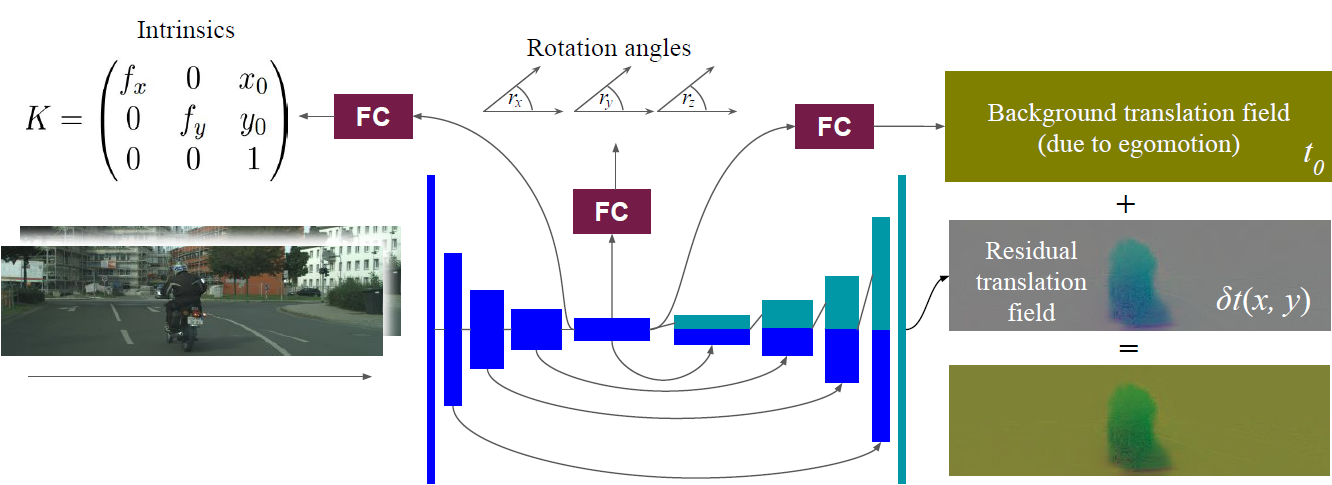
\includegraphics[width=1\linewidth]{imgs/2.png} 
  \caption{运动预测网络的示意图。}
  \end{framed}
\end{figure*}
\subsection{losses}
基于估计的深度图,相机内参,旋转和平移场,我们重投影第一个帧以匹配第二个帧,并使用两个损失进行比较:1)结构相似度(SSIM)损失;2)颜色通道的L1距离之和[6]。另外,我们通过估计向前和向后运动对运动场施加周期一致性损失,这是通过将两帧的顺序以正向和反向输入网络而获得的。消除掉相机运动的影响,那些场景运动所涉及的像素在调换帧顺序之后会表现出相反的运动,因此我们根据相对旋转和平移的相对偏差定义了L2损失。此外,我们对深度和运动场应用空间L1平滑度损失,对深度应用时间L1平滑度损失,以及L2权重正则项。补充材料中提供了更多详细信息。

\subsection{Occlusion-aware consistency}
当相机和物体移动时,在一帧中可见的区域可能会在另一帧中被遮挡。不能在与这些区域相对应的像素中强制执行光度一致性。给定一幅深度图和一帧运动场,则实际上可以检测出将发生遮挡的位置,并将遮挡区域排除在一致性损失之外。检测被遮挡的像素需要某种关于深度图表示的表面的连通性和z缓冲的推理。要保持该机制的可微并在插入训练循环后具有足够的效率是有挑战的。
\begin{figure}[htbp]
  \begin{framed}
  \centering
    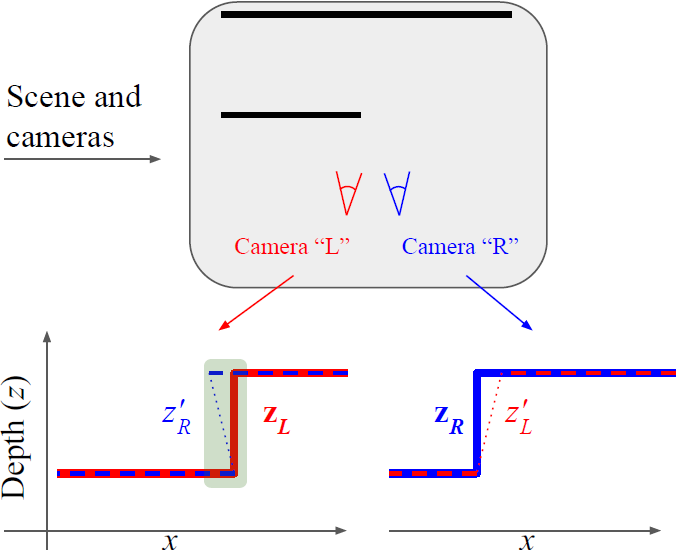
\includegraphics[width=1\linewidth]{imgs/3.png} 
  \caption{处理遮挡的方法在顶部,我们显示了一个二维“场景”,它由两个直的表面组成,一个部分遮挡另一个左右两台摄像机正在观察场景我们的方法是单目的,因此它们代表同一台移动相机的两个位置,为方便起见使用“左”和“右”在底部,每个摄像头观察到的深度图在相应侧面($z_L$和$z_R$)上以实线表示虚线表示从一个视图重投影到另一个视图($z'_R$和$z'_L$)获得的深度图重投影深度图可能有多个值,表示遮挡(请参见绿色阴影的矩形)为了解决这个问题,我们仅将光度损失和几何损失应用于$z'_R\leq z_L$和$z'_L\leq z_R$的像素当深度图和运动估计正确时,此方案中的损失值为零。}
\end{framed}
\end{figure}
因此,我们采用了不同的方法,如图3所示。对于源帧中的每个像素$(i,j)$,利用预测深度$z_{ij}$和相机内参矩阵获取空间中的相应点$(x_{ij},y_{ij},z_{ij})$,该点根据预测的运动场在空间中移动。特别地,深度变为$z'$。新的空间位置被重新投影到相机视角,并落在位置$(i',j')$。$i'$和$j'$通常是非整数。因此,要获得目标帧在$(i',j')$处的深度$z^{t}_{i',j'}$,需要进行插值。

遮挡发生在$z'$变为多值的$(i',j')$处。在这种情况下,颜色和深度一致性应仅应用于$z'$的可见分支,即$z'$较小的分支。如果源帧和目标帧几乎一致,则可见分支将在$(i',j')$处接近目标深度$z^{t}_{i',j'}$。我们建议选择可见分支的方法是在损失函数中仅包括$z'_{i',j'}≤z^{t}_{i',j'}$的点$(i',j')$。换句话说,只有当源帧的变换像素落在目标帧中的深度图的前面时,我们才将该像素包括在损失函数中。这种方案在交换源帧和目标帧方面不是对称的,这就是为什么我们始终以对称方式应用它的原因:我们将源帧投影到目标帧上,计算损失,然后交换源和目标帧再计算一次。图3给出了该方法。

第4.2节中所述的周期一致性损失就是以本节所述的“遮挡感知”方式计算。但对于SSIM我们通过用加权平均替换所有平均操作来处理遮挡,其中像素的权重是该像素中深度误差的递减函数。确切的表达式在SM中给出。

\subsection{Regularization}
\subsubsection{translation field的语义正则化}
等式(1)可以将帧不一致性损失传播到每个像素的$z$,$R$和$t$。但是,如果不进行进一步的规范化处理,它们的功能仍然很不确定。尽管$z$,$R$和$t$的连续性是强大的正则化器,但我们发现进一步的正则化有很大帮助。特别地,我们在整个图像中强加R的恒定性,并允许$t$仅在指定为可能移动的像素处偏离恒定值。与先前的工作[6]不同,不需要实例分割和跟踪,因为我们需要的只是一个“可能移动的”掩码$m(x,y)$。我们定义:
\begin{equation}
  t(x,y)=t_0+m(x,y)\delta(x,y)
\end{equation}
其中$t_0$是由于相机运动造成的“背景运动”,$\delta(x,y)$是由于场景运动造成的“残差运动”。

消融实验表明,$m(x,y)$可以像边界框的并集一样粗糙(参见图4)。此外,将L1平滑算子应用于$t(x,y)$。
\subsubsection{Randomized layer normalization}
在我们的实验中,我们观察到与批规范化(BN)相关的以下异常行为:
\begin{itemize}
  \item 在BN的“训练模式”下进行推断时,评估指标始终更好。就是说,与其使用长期的平均均值和方差,不如使用在推理过程中从图像本身获得的均值和方差\footnote{Even at batch size 1, there would still be means and variances over the spatial dimensions.},这个时候使批归一化更类似于层归一化[3]。
  \item 随着batch size的增加,无论如何缩放学习率,评估准确性始终越来越差。
\end{itemize}

这两个异常得出的结论是,BN的行为就像层归一化(LN)[3]一样,对于batch中的每个项目,其他项目都充当噪声源。用带有乘性高斯噪声的LN代替BN可以改善评估指标,并且随着batch size的增加(同时线性的增加学习率[14])而不会造成性能损失,甚至评估指标略有改善。

\subsection{Learning the intrinsics}
如式(1)所示,相邻帧之间的光度一致性损失为$K$提供了一个监督信号,但仅当它们之间的摄像机旋转非零即$R\neq\mathbb{E}$时。当$R=\mathbb{E}$时。(1)变为$z'p'= zp + Kt$,这意味着损失函数仅取决于乘积$Kt$。但是,即使$K$和$t$不正确,$Kt$也可以完全正确。实际上,对于任何非奇异的$\tilde{K}$,都存在$\tilde{t} =\tilde{K}^{-1}Kt$,从而$\tilde{K}\tilde{t}= Kt$。尤其是当$K$和$t$由来自同一网络的预测时,只要预测乘积正确的$K$和$t$,网络就可以“逃避”监视信号。

幸运的是,旋转可以为K提供监视信号。公式(3)(详见补充材料)将确定焦距的容差(以像素为单位的$\delta f_x$和$\delta f_y$)与相机旋转量联系起来:
\begin{equation}
  \delta f_x < \frac{2f_x^2}{wsr_y};\delta f_y < \frac{2f_y^2}{hsr_x};
\end{equation}
其中$r_y$和$r_x$是相应轴的旋转角度,$w$和$h$分别是图像的宽度和高度,并且$s = max(h,w)$。

\section{Experiments}
在本节中,我们评估了深度预测,里程计估计以及各种数据集上的相机内参数估计的性能。
\subsection{Datasets}
\textbf{KITTI} 数据集是在城市环境中收集的,是深度和自我运动估计的主要基准。它带有一个LIDAR传感器,仅用于评估。我们将数据集拆分为训练、验证和测试集,通常称为Eigen split。KITTI使用了39835个培训示例。

\textbf{Cityscapes} 数据集是更新的城市驾驶数据集,我们将其用于训练和评估。这是一个具有许多动态场景的更具挑战性的数据集。除了少数例外[27,6],它尚未用于深度估计评估。它包含38675个培训示例。我们使用视差数据中的深度对1250个样本的标准评估集进行评估[27,6]。

\textbf{EuRoC Micro Aerial Vehicle Dataset} 数据集[5]是室内飞行器收集的非常具有挑战性的数据集。虽然数据包含一整套传感器测量值,包括双目图像、IMU、准确的Leica激光跟踪仪生成的GT,Vicon场景3d扫描和相机校准数据,但我们仅使用单目视频进行训练。由于相机的镜头畸变很大,因此这是测试我们学习镜头变形的方法的机会。

\textbf{YouTube8M} 为了证明可以从未知的摄像机中获取野外视频的深度,我们从YouTube8M数据集中收集了视频[1]。从YouTube8M的3079个带有“quadcopter”标签的视频中,人类评分者选择了包含大量来自四轴飞行器的镜头的视频。当然,这些视频是使用不同的未知相机拍摄的,具有不同的视野和不同程度的镜头失真。补充材料中列出了YouTube8M ID。

\subsection{Depth}
由于单目方法只能估计全局比例因子下的深度,因此,我们遵循该领域的常规做法[47],根据预测深度和GT的中值对比例因子进行归一化(code)。

\textbf{KITTI} 表1总结了在KITTI上训练的模型对KITTI Eigen partition的评估结果。度量标准是在Zhou等人中定义的[47]。表1仅显示最佳方法和前三个指标,其余在SM中给出。如表中所示,我们改进了最新结果。更重要的是,我们观察到,学习内参而不是给定内参有助于性能提升。
\begin{table}
  \centering
  \begin{tabular}{|c|c|c|c|c|}
  \hline
  Method&M&Abs Rel&Sq Rel& RMSE\\
  \hline
  Zhou [47]       &  &  0.208& 1.768& 6.856\\
  Yang [42]       &  &  0.182& 1.481& 6.501\\
  Mahjourian [24] &  &  0.163& 1.240& 6.220\\
  LEGO [41]       & √&  0.162& 1.352& 6.276\\
  GeoNet [44]     & √&  0.155& 1.296& 5.857\\
  DDVO [35]       &  &  0.151& 1.257& 5.583\\
  Godard [13]     &  &  0.133& 1.158& 5.370\\
  Struct2Depth [6]& √&  0.141& 1.026& 5.291\\
  Yang [40]       &  &  0.137& 1.326& 6.232\\
  Yang [40]       & √&  0.131& 1.254& 6.117\\
  \hline
  Ours:&&&&\\
  Given intrinsics& X& 0.129& 0.982& 5.23\\
  Learned intrinsics& X &0.128& 0.959& 5.23\\
  \hline
  \end{tabular}
  \caption{KITTI上的对比,“M”列有标记的考虑了对象运动,最大深度80m。}
\end{table}

\textbf{Cityscapes} 表2总结了在Cityscapes上训练和测试的模型的评估指标。我们参考以前的工作,使用视差进行评估[6,27]。由于Cityscapes具有许多动态对象,非常具有挑战性,因此很少有方法使用这个数据集进行评估。如表2所示,我们的方法优于以前的方法,并从学习内参中受益。
\begin{table}
  \centering
  \begin{tabular}{|c|c|c|c|c|}
  \hline
  Method&M&Abs Rel&Sq Rel& RMSE\\
  \hline
  Pilzer [27]         & & 0.440& 5.713& 5.443\\
  Struct2Depth [6]    &X& 0.145& 1.736& 7.279\\
  \hline
  Ours:&&&&\\
  Given intrinsics    &X& 0.129& 1.35 & 6.96\\ 
  Learned intrsinsics &X& 0.127& 1.33 & 6.96\\ 
  \hline
  \end{tabular}
  \caption{Cityscapes上的对比,“M”列有标记的考虑了对象运动,最大深度80m。}
\end{table}

\textbf{Cityscapes+KITTI} 无需相机内参就能学习深度,从而为从任何数据源提供了机会。图5显示了合并Cityscapes和KITTI数据集并对其进行评估的结果。在该实验中,假定内参是未知的,通过学习获得。对两个数据集进行联合训练可改善深度指标,甚至超过分别在两个数据集上获得的最佳结果。这是一个关键结果,证明了我们的方法能够利用可能无限大小的数据源。
\begin{figure}[htbp]
  \begin{framed}
     \centering
       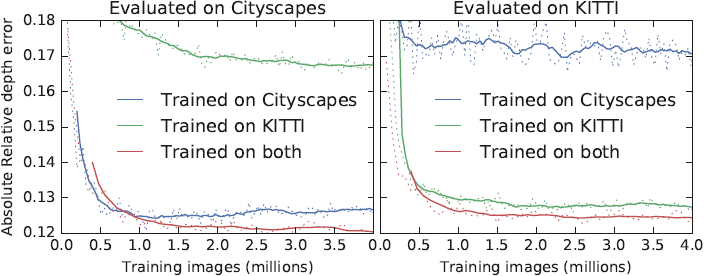
\includegraphics[width=1\linewidth]{imgs/5.png} 
     \caption{对Kitti和Cityscapes的深度预测。将两个数据集结合在一起可以改善两个结果。学习内参可以提高泛化能力,即使它们来自未知相机。}
  \end{framed}
  \end{figure}

\textbf{Cityscapes+KITTI: ablation experiments}表3总结了我们为了研究本文描述的每种技术对最终结果的影响而进行的消融实验的结果。为了减少结果组合的数量,在所有实验中,训练集都是将Cityscapes和KITTI混合在一起。每个模型分别在Cityscapes和KITTI上进行了评估。
\begin{table}
  \centering
  \begin{tabular}{|c|c|c|}
  \hline
  &\multicolumn{2}{c|}{Abs Rel depth}\\
  Experiment& CS& KITTI\\
  \hline
  Our algorithm &0.121& 0.124\\
  \hline
  Boxes instead of segmentation masks& 0.120& 0.125\\
  w/o occlusion-aware loss& 0.127& 0.126\\
  w/o object motion& 0.172& 0.130\\
  w/o randomized layer normalization& 0.124& 0.127\\
  \hline
  \end{tabular}
  \caption{深度估计的消融实验。在所有实验中,训练集都是Cityscapes(CS)和KITTI的组合,我们分别在Cityscapes(CS)和KITTI(特征分区)上测试了该模型。每行代表一个实验,与主要方法相比,只做了一个更改,如“实验”行中所述。数字越小越好。}
\end{table}

\begin{figure}[htbp]
  \begin{framed} 
  \centering
    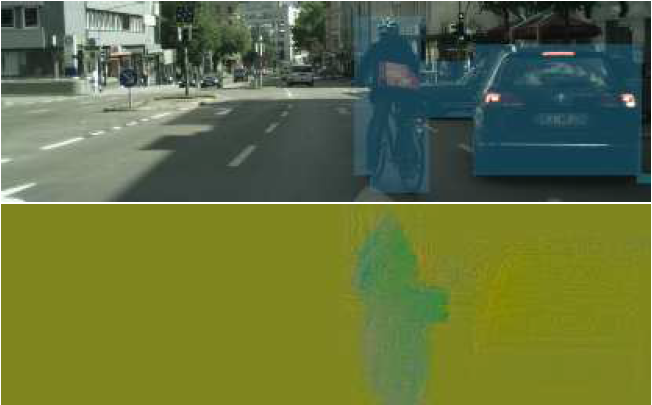
\includegraphics[width=1\linewidth]{imgs/4.png} 
  \caption{使用“possibly mobile”掩码来规范translation field物体检测网络识别行人、骑自行车的人和汽车等能够运动的物体边界框的并集形成“possibly mobile”掩码顶部的图片来自Cityscapes,标明了掩码的,底部的图片是网络预测的translation field(x,y,z编码为RGB)金色背景对应于负z方向的运动,因为整个场景都朝着相机移动绿色的轮廓是骑车人稍微向左和朝着相机移动请注意,网络将轮廓从粗糙的蒙版中雕刻出来。}
  \end{framed}
\end{figure}


使用边界框的并集作为“可能移动的像素”掩码(如图4所示)与使用分割掩码一样好,这使我们的技术更广泛地适用。物体运动估计显示出至关重要的作用,特别是在Cityscapes上,其特征是场景更加复杂,行人和汽车也更多。随机LN被证明比标准BN更好。遮挡感知提高了深度估计的质量,尤其是在Cityscapes上,该场景具有丰富的场景和更多的遮挡。图6可视化了遮挡感知的影响。
\begin{figure}[htbp]
\begin{framed}
     \centering
       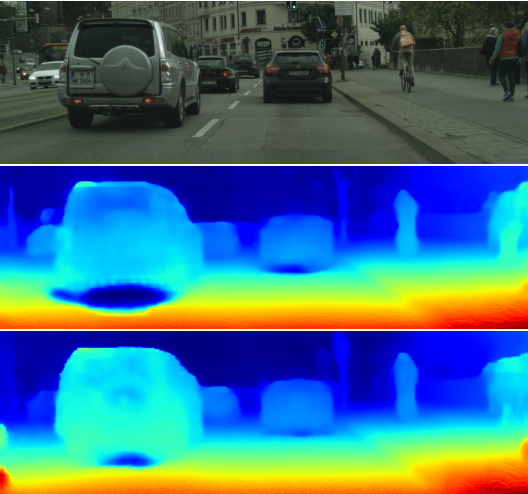
\includegraphics[width=1\linewidth]{imgs/6.png} 
     \caption{遮挡感知损失的效果。中图和底图是从上图获得的视差图。中图没有使用遮挡感知。在汽车下方被遮挡的区域,遮挡感知损失可减少伪影。上图属于Cityscapes测试集,并且是遮挡感知效果较强的图像之一。}
    \end{framed}
\end{figure}

\textbf{EuRoC MAV Dataset}我们进一步使用EuRoC MAV数据集来评估深度。选择了一个极富挑战性的out-of-sample评估方案,该方案中我们对“Machine room”序列进行了训练,并在具有3D GT的“Vicon Room 2 01”上进行了测试。表4报告了结果。补充材料详细介绍了如何通过提供的Vicon 3D扫描生成深度GT。
\begin{table}
  \centering
  \begin{tabular}{|c|c|c|c|c|c|c|}
  \hline
  Abs R& Sq R& RMS &lgRMS& a1& a2& a3\\
  \hline
  0.332& 0.389& 0.971& 0.396& 0.420& 0.743& 0.913\\
  \hline
  \end{tabular}
  \caption{EuRoC数据集的深度估计,该数据集没有可对比的先前结果。 $a_i = \delta <1.25^i$。}
\end{table}
\subsection{YouTube Videos}
为了证明可以从任意相机参数未知的视频中预测深度,我们在5.1节中介绍的YouTube8M视频数据集上训练了我们的模型。图7将结果可视化。我们注意到,该数据集具有很大的深度范围,因此具有很大的挑战性。
\begin{figure}[htbp]
  \begin{framed}
     \centering
       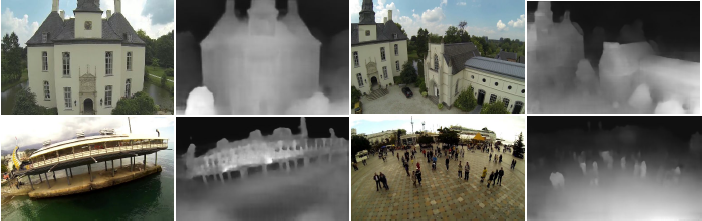
\includegraphics[width=1\linewidth]{imgs/7.png} 
     \caption{YouTube视频的深度预测结果,相机内参也是通过网络预测的。}
  \end{framed}
\end{figure}
\subsection{Camera intrinsics evaluation}
在评估我们的方法学习相机内参的性能时,可以提出两个单独的问题。首先,帧间一致性为相机内参提供的监控信号有多好。其次是深度网络在学习它们和推广测试数据方面的表现如何。
\begin{table}
  \centering
  \begin{tabular}{|c|c|c|}
  \hline
  Quantity& Learned& GT\\
  \hline
  Horizontal focal length (fx)&   253.7 ± 1.1  &  250.2\\
  Vertical focal length (fy)  &   265.4 ± 1.3  &  261.3\\
  Horizontal center (x0)      &   189.0 ± 0.9  &  187.2\\
  Vertical center (y0)        &   132.2 ± 1.1  &  132.8\\
  Quadratic radial distortion &  −0.267 ± 0.003& −0.283\\
  Quartic radial distortion   &   0.064 ± 0.002&  0.074\\
  \hline
  \end{tabular}
  \caption{在EuRoC数据集上学习的相机内参。仅使用单目图像(“cam0”)在11个数据集中分别进行了深度、自我运动和内参的学习。分别收集每个内参变量的统计信息(均值和标准差)。将GT调整为适应图像大小(256×384)。}
\end{table}

\textbf{监督信号的质量} 为了评估内在函数的监督信号,我们将每个内参表示为一个单独的学习变量。这适用于EuRoC数据集,因为整个数据集都是使用同一相机捕获的。EuRoC的11个子集中的每个子集都在单独的实验中接受训练,产生11个独立的结果。表5总结了每个内参的所得样本均值和标准差。所有参数在几个像素内与groundtruth一致。由于GT值未附带公差,因此很难确定差异是否在公差范围内。视差图如图8所示。
\begin{figure}[htbp]
  \begin{framed}
     \centering
       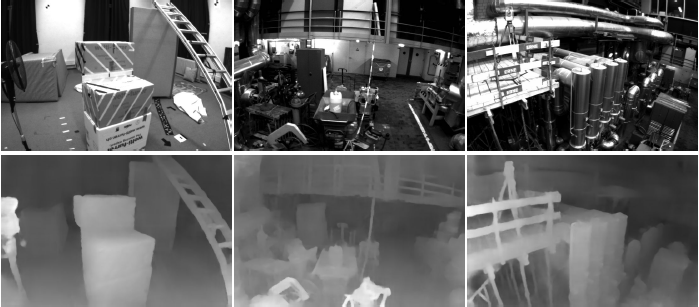
\includegraphics[width=1\linewidth]{imgs/8.png} 
     \caption{RuRoC的深度预测结果,相机内参也是通过网络预测的。}
  \end{framed}
\end{figure}

\textbf{泛化能力} 先前的工作[37,39,4]已经表明,深度网络可以在严格监督的情况下学习和概括相机的内参。在我们的设置中,相机的内参和运动是由同一网络预测的,因此相互关联。换句话说,施加在运动/内参网络上的损失函数仅在等式(3)的限制内强加了内参的正确性。

我们评估了模型对KITTI odometry的内参的预测。该模型是在Cityscapes和KITTI训练集的上进行训练的,它们的典型焦距明显不同。图9显示了预测fx随ry的函数的散布图。这些预测处于等式(3)的限制之内。虽然表5给出了用于内参的高质量监视信号,但图9显示,当同一网络预测内在函数和运动时,后者会“整体”学习它们, 仅在深度预测网络学习深度所需的程度上。
\begin{figure}[htbp]
  \begin{framed}
     \centering
       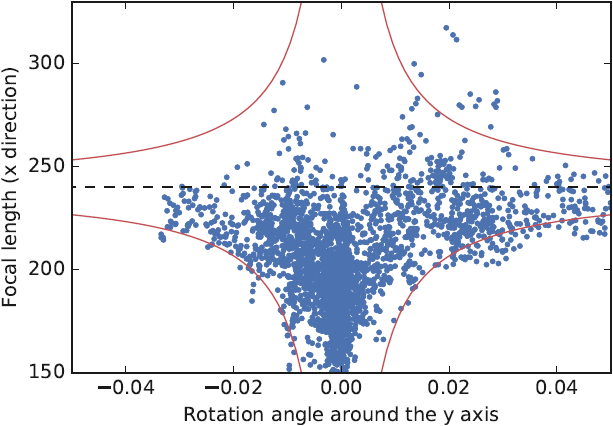
\includegraphics[width=1\linewidth]{imgs/9.png} 
     \caption{KITTI odometry序列09和10中的所有图像,预测的$f_x$是预测$r_y$的函数。红色曲线显示了等式3施加的公差极限,虚线是groundtruth。}
  \end{framed}
\end{figure}

\subsection{Odometry}
我们在KITTI序列09和10上评估了相机自我运动预测。常见的5点绝对轨迹误差(ATE)度量[47、6、44、13]用于测量估算轨迹与相应GT之间的局部一致性。但是,评估一种定位方法的有用性需要评估其在预测位置中的准确性。定位的一个通用指标是平均相对平移 $drift_{trel}$ [31,46] –预测位置与GT位置之间的距离除以在轨迹上行进的距离平均。表6总结了这两个指标,证明了我们的方法在这两个方面都实现了改进

\begin{table}
  \centering
  \begin{tabular}{|c|c|c|c|c|}
  \hline
  &\multicolumn{2}{c|}{Seq.09}&\multicolumn{2}{c|}{Seq.10}\\
  \cline{2-5}
  Metric& ATE& $t_{rel}$ &ATE& $t_{rel}$\\
  \hline
  Zhou [47]         &  0.021& 17.84\%& 0.020& 37.91\%\\
  GeoNet [44]       &  0.012&   /    & 0.012&   /    \\
  Zhan [46]         &    /  & 11.92\%&   /  & 12.45\%\\
  Mahjourian [24]   &  0.013&   /    & 0.012&   /    \\
  Struct2depth [6]  &  0.011&  10.2\%& 0.011& 28.9\% \\
  \hline
  Ours, with intrinsics:&&&&\\
  Learned             & 0.012& 7.5\%& 0.010& 13.2\%\\
  Learned \& corrected& 0.010& 2.7\%& 0.007&  6.8\%\\
  Given               & 0.009& 3.1\%& 0.008&  5.4\%\\
  \hline
  \end{tabular}
  \caption{KITTI odometry 09和10序列上的绝对轨迹误差(ATE)[47]和平均相对平移漂移($t_{rel}$)[31]。 }
\end{table}

在评估里程表时,最幼稚的方法是为每对相邻帧计算自我运动的推断。这导致了图10中的红色“learned intrinsics”曲线。但是,如果我们在推理时知道相机的参,也可以进行推理时校正。在这种情况下,可以利用以下事实:对于旋转角度和焦距的小误差,$r_x f_y$和$r_y f_x$近似恒定(等式SM8)。因此,如果网络为给定的一对图像预测了$r'_y$和$f'_x$,并且我们知道了真实的焦距$f_x$,则可以将$r_y$的估计值校正为$r'_yf'_x / f_x$。这是在图10中生成“Learned and corrected intrinsics”曲线时所调用的过程,以及表6中的相应条目。在经过推理时校正的情况下,使用GT内参和学习内参得到的轨迹结果类似。两者有均显着改善,如$t_{rel}$度量所表明的那样。
\begin{figure}[htbp]
  \begin{framed}
     \centering
       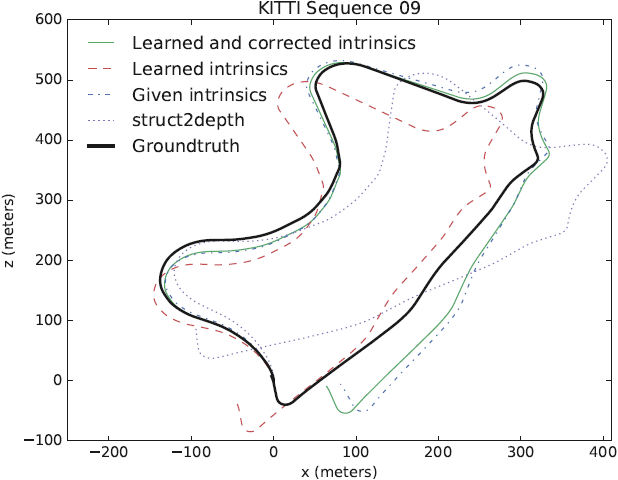
\includegraphics[width=1\linewidth]{imgs/10.png} 
     \caption{KITTI odometry序列09上的轨迹预测。}
  \end{framed}
\end{figure}

\section{Conclusions}
这项工作通过对遮挡物进行几何处理,一种简单的解决物体运动的方法以及一种新颖的正则化形式,解决了对深度和视觉里程计进行无监督学习的重要挑战。最重要的是,它朝着利用大量现有的未标记视频进行学习深度评估迈出了重要一步:通过无监督学习相机参数(包括镜头畸变),它首次实现了从未知相机拍摄的原始视频中学习深度。


% use section* for acknowledgment
\ifCLASSOPTIONcompsoc
  % The Computer Society usually uses the plural form
  \section*{Acknowledgments}
\else
  % regular IEEE prefers the singular form
  \section*{Acknowledgment}
\fi
%%致谢
We Thank Roland Siegwart for the permission to use EuRoC dataset, Sergey Ioffe for enlightening discussions about batch normalization, Jason Su and Kwea Koi for spotting an error in the derivation in an earlier version of the manuscript, Kurt Konolige for consultation and critical reading of the manuscript, and Chad Richards for copyediting the paper.

\cleardoublepage
\section*{补充材料}
\subsection*{A.1.关于相机内参的推导}
在本节中,我们推导出方程式3,以估计旋转提供的用于学习相机内部特性的监督信号的准确性。令R和t为两帧之间发生的旋转和平移,而K为内参矩阵:
\begin{equation}
  K = \begin{pmatrix}
    f_x & 0 & x_0\\
    0 & f_y & y_0\\
    0  &  0  &  1
  \end{pmatrix}
  \tag{SM1}
\end{equation}
对于第一帧中的每个像素位置$p$,等式(1)提供了由于$R$和$t$而产生的偏移位置$p'$。

光度误差项提供$p'$的监控信号。因此,只要它们产生正确的$p'$,它们就不会区分$R$,$t$和$K$的组合。令$\tilde{R}$,$\tilde{t}$和$\tilde{K}$为$R$,$t$和$K$的一组可能不正确的预测。如果我们能够满足:
\begin{equation}
  KRK^{-1}zp+Kt=\tilde{k}\tilde{R}\tilde{k}^{-1}zp+\tilde{k}\tilde{t}
  \tag{SM2}
\end{equation}
那么$\tilde{R}$,$\tilde{t}$和$\tilde{K}$就与$R$,$t$和$K$相等了。

如第4.4节所述,总存在$\tilde{t}$,使等式SM2中的$Kt$和$\tilde{k}\tilde{t}$相互抵消。因此,以后将省略平移。$z$也可以消掉,这在直觉上是有意义的,因为对于针孔相机,在没有平移的情况下,由于旋转而导致的像素空间的移动量仅取决于旋转,而不取决于对象和相机的距离。

p的齐次坐标可以表示为$(p_x, p_y, 1)$,其中$p_x$和$p_y$是像素坐标系中的坐标。旋转后,$p_x$将移至:
\begin{equation}
  p'_x=\frac{(KRK^{-1}p)_1}{(KRK^{-1}p)_3};\tilde{p}'_x=\frac{(\tilde{K}\tilde{R}\tilde{K}^{-1}p)_1}{(\tilde{K}\tilde{R}\tilde{K}^{-1}p)_3};
  \tag{SM3}
\end{equation}
两种表达形式取决于我们使用$K$和$R$还是$\tilde{K}$和$\tilde{R}$tilde下标1和3表示通过将3x3矩阵$KRK_{-1}$或$\tilde{K}\tilde{R}\tilde{K}^{-1}$乘以三维矢量p得到的三维矢量的各个分量tilde$p'_y$和$\tilde{p}'_y$具有类似的表达式,只需将下标1替换为2。

在下文中,我们仅考虑较小的旋转,因为通常只有在旋转足够小以允许旋转前后的视场之间有足够的重叠时,才可能在两个帧之间使用光度一致性,并且因为小角度近似有助于推导简单的解析方程,如等式(3)。

我们将$R$写成$\mathbb{E}+r$,其中$r$为:
\begin{equation}
  r = \begin{pmatrix}
      0 & r_z&-r_y\\
    -r_z&  0 & r_x\\
     r_y&-r_x&  0    
  \end{pmatrix}
  \tag{SM4}
\end{equation}
$\tilde{R}$与之类似。对公式(SM3)中的$r$进行泰勒级数展开:
\begin{equation}
  p'_x=p_x+(KrK^{-1}p)_1-p_x(KrK^{-1}p)_3
  \tag{SM5}
\end{equation}
$\tilde{p}'_x$的情况类似。

将公式(SM1)和公式(SM4)代入公式(SM5),得到:
\begin{multline}
  p'_x=-f_xr_y-r_y\frac{(p_x-x_0)^2}{f_x}+\\
  r_x\frac{(p_x-x_0)(p_y-y_0)}{f_y}+r_z\frac{(p_y-y_0)f_x}{f_y}
  \tag{SM6}
\end{multline}
\begin{multline}
  p'_y=f_yr_x+r_x\frac{(p_y-y_0)^2}{f_y}-\\
  r_y\frac{(p_x-x_0)(p_y-y_0)}{f_x}-r_z\frac{(p_x-x_0)f_y}{f_x}
  \tag{SM7}
\end{multline}
$\tilde{p}'_x$和$\tilde{p}'_y$的情况类似。

我们假设$K$和$R$的预测误差远小于1个像素,不会影响光度误差,导致无法通过光度误差损失函数将这种预测误差消除。因此,我们需要导出$\tilde{R}$和$\tilde{K}$的表达式,满足$|\tilde{p}'_x-p'_x|\ll1$,$|\tilde{p}'_y-p'_y|\ll1$。

公式(SM6)和(SM7)为对$K$和$R$进行全面误差分析提供了基础,但是全面分析超出了本文的范围。相反,我们将讨论限于焦距的误差分析。假设网络错误地预测了$f_x$和$f_y$,取而代之的是$\tilde{f}_x$和$\tilde{f}_y$。由于相同的网络可以预测$R$,因此我们假设它选择了$\tilde{R}$,以消除错误预测的$f_x$和$f_y$的某些影响。为简单起见,我们选择$R$,使得至少在光轴上的像素$(p_x=x_0, p_y=y_0)$处,$p'_x$和$p'_y$保持不变。从等式(SM6)和(SM7)可以看到,这需要:
\begin{equation}
  \tilde{r}_y=r_y\frac{f_x}{\tilde{f}_x},\tilde{r}_x=r_x\frac{f_y}{\tilde{f}_y}
  \tag{SM8}
\end{equation}
We can now write the $tilde$ version Eqs. SM6 and SM7($tilde$ version for $p$ is $\tilde{p}$), using rprime to eliminate $\tilde{r}_x$ and $\tilde{r}_y$ form the equations. The result is:
\begin{multline}
  \tilde{p}'_x=-f_xr_y-r_yf_x\frac{(p_x-x_0)^2}{(\tilde{f}_x)^2}+\\
  r_xf_y\frac{(p_x-x_0)(p_y-y_0)}{(\tilde{f}_y)^2}+r_z\frac{(p_y-y_0)\tilde{f}_x}{\tilde{f}_y}
  \tag{SM9}
\end{multline}
\begin{multline}
  \tilde{p}'_y=f_yr_x+r_xf_y\frac{(p_y-y_0)^2}{(\tilde{f}_y)^2}-\\
  r_yf_x\frac{(p_x-x_0)(p_y-y_0)}{(\tilde{f}_x)^2}-r_z\frac{(p_x-x_0)\tilde{f}_y}{\tilde{f}_x}
  \tag{SM10}
\end{multline}
令$\tilde{p}'_x=p'_x+\delta p'_x$,$\tilde{f}_x=f_x+\delta f_x$,$y$的情形类似。结合公式(SM6)、(SM7)、(SM9)、(SM10),得到:
\begin{multline}
  \delta p'_x =2r_y\delta f_x\frac{(p_x-x_0)^2}{(f_x)^2}
  -2r_x\delta f_y\frac{(p_x-x_0)(p_y-y_0)}{(f_y)^2}\\
  +r_z\frac{(p_y-y_0)f_x}{f_y}\left(\frac{\delta f_x}{f_x}-\frac{\delta f_y}{f_y}\right)
  \tag{SM11}
\end{multline}
\begin{multline}
  \delta p'_y =-2r_x\delta f_y\frac{(p_y-y_0)^2}{(f_y)^2}
  +2r_y\delta f_x\frac{(p_y-y_0)(p_x-x_0)}{(f_x)^2}\\
  -r_z\frac{(p_x-x_0)f_y}{f_x}\left(\frac{\delta f_y}{f_y}-\frac{\delta f_x}{f_x}\right)
  \tag{SM12}
\end{multline}
其中$f_x$和$f_y$中高于一阶的项已被删除。

公式(SM11)和(SM12),以及$|\delta p'_x|\ll 1$和$|\delta p'_y|\ll 1$的要求,可用于估计给定任意小旋转$r$的$\delta f_x$和$\delta f_y$的边界。为了深入了解公式SM11和SM12,在下面的内容中,我们推导了在r的三个分量(即围绕x、y和z轴的旋转)中有两个为零的情况下$\delta f_x$和$\delta f_y$的边界的显式表达式。

\textbf{Rotations around the $z$ axis}
如果只有$r_z$非0,考虑到$|\delta p'_x|\ll 1$且$|\delta p'_y|\ll 1$,公式(SM11)和公式(SM12)可以化简为:
\begin{align*}
  \centering
  &\left|\frac{\delta f_y}{f_y}-\frac{\delta f_x}{f_x} \right|\ll \frac{f_x}{r_zf_y\left|p_x-x_0\right|}\\
  &\left|\frac{\delta f_y}{f_y}-\frac{\delta f_x}{f_x} \right|\ll \frac{f_y}{r_zf_x\left|p_y-y_0\right|}
  \tag{SM13}
\end{align*}
如果$f_y$和$f_x$处于相同的数量级,并且$x_0\approx w/2$,$y_0\approx h/2$,那么(SM13)就能化简为:
\begin{align*}
  \centering
  &\left|\frac{\delta f_y}{f_y}-\frac{\delta f_x}{f_x} \right|\ll \frac{f_x}{wr_z}\\
  &\left|\frac{\delta f_y}{f_y}-\frac{\delta f_x}{f_x} \right|\ll \frac{f_y}{hr_z}
  \tag{SM14}
\end{align*}
我们可以从(SM13)和(SM14)中发现,绕Z轴的旋转:
\begin{itemize}
  \item $r_z$能限制$f_x$和$f_y$之间的比率。
  \item $r_z$不能提供对$f_x$和$f_y$的监督信号。
  \item 监督信号的强度与旋转的大小和图像的高度/宽度(以像素为单位)成反比。
\end{itemize}

\textbf{Rotations around the $y$ axis}
如果只有$r_y$非0,考虑到$|\delta p'_x|\ll 1$且$|\delta p'_y|\ll 1$,公式(SM11)和公式(SM12)可以化简为:
\begin{align*}
  &|\delta f_x| \ll \frac{(f_x)^2}{2r_y(p_x-x_0)^2}\\
  &|\delta f_x| \ll \frac{(f_x)^2}{2r_y|p_y-y_0||p_x-x_0|}
  \tag{SM15}
\end{align*}
与前面的过程类似,距离中心最远的像素为$|\delta f_x|$提供了边界。如果$x_0\approx w/2$,$y_0\approx h/2$,则(SM15)可以表示为:
\begin{equation*}
  |\delta f_x|\ll min\left(\frac{2f_x^2}{r_yw^2},\frac{2f_x^2}{r_ywh}\right)
  \tag{SM15.5}
\end{equation*}
从(SM15)和(SM15.5)中发现,绕Y轴的旋转:
\begin{itemize}
  \item 为$f_x$提供监督信号。
  \item 监控信号的大小与旋转角的大小和图像的高度/宽度的平方成反比。
\end{itemize}

由于绕x轴旋转会推出与(SM15.5)相同的表达式,其中$x$和$y$互换,$w$和$h$互换。综上所述,即可得出等式(3)。

\subsection*{A.2.相机运动和内参预测网络}
该网络的示意图如图2所示。步长为2的卷积层串联形成编码器,最后连接一个平均池化,形成了1024个通道的bottleneck,其空间分辨率为1x1。从bottleneck出发,有以下几个分支:
\begin{itemize}
  \item 全连接层,具有3个输出,分别是全局旋转角度($r_0$)和全局平移矢量($t_0$)。后两个代表由于摄像机运动而导致整个场景相对于摄像机的运动。
  \item 通过1x1卷积预测每个内参分量。Softplus激活可保持焦距为正值,并且保证畸变曲线单调增加。
  \item 解码器预测具有3个输出通道的密集残差平移矢量场t(x,y),表示每个像素相对于场景的3D运动。每个解码器层接收前一个解码器层的输出和遵循UNet架构的相应编码器层的输出作为输入。
\end{itemize}

对于表5中所示每个参数,都分配给一个单独的可训练变量,而不是从网络中预测内参。这是合并所有训练示例的内在函数都应相同的约束的一种方法,因为整个EuRoC数据集是使用同一台摄像机捕获的。失真变量初始化为零,$x_0$和$f_x$初始化为$w/2$,$y_0$和$f_y$初始化为$h/2$。
\cleardoublepage
\begin{table*}
  \centering
  \begin{tabular}{|c|c|c|c|c|c|c|c|c|}
  \hline
  Method&M&Abs Rel&Sq Rel&RMSE&RMSE log&$\delta<1.25$&$\delta<1.25^2$&$\delta<1.25^3$\\
  \hline
  Zhou [47]        & & 0.208& 1.768& 6.856& 0.283& 0.678& 0.885& 0.957\\
  Yang [42]        & & 0.182& 1.481& 6.501& 0.267& 0.725& 0.906& 0.963\\
  Mahjourian [24]  & & 0.163& 1.240& 6.220& 0.250& 0.762& 0.916& 0.968\\
  LEGO [41]        &√& 0.162& 1.352& 6.276& 0.252& 0.783& 0.921& 0.969\\
  GeoNet [44]      &√& 0.155& 1.296& 5.857& 0.233& 0.793& 0.931& 0.973\\
  DDVO [35]        & & 0.151& 1.257& 5.583& 0.228& 0.810& 0.936& 0.974\\
  Godard [13]      & & 0.133& 1.158& 5.370& 0.208& 0.841& 0.949& 0.978\\
  Struct2Depth [6] &√& 0.141& 1.026& 5.291&0.2153&0.8160&0.9452&0.9791\\
  Yang [40]        & & 0.137& 1.326& 6.232& 0.224& 0.806& 0.927& 0.973\\
  Yang [40]        &√& 0.131& 1.254& 6.117& 0.220& 0.826& 0.931& 0.973\\
  \hline
  Ours:              & &  &  &  &  &  &  &  \\
  Given intrinsics   &√& 0.129& 0.982& 5.23& 0.213& 0.840& 0.945& 0.976\\
  Learned intrinsics &√& 0.128& 0.959& 5.23& 0.212& 0.845& 0.947& 0.976\\
  \hline
\end{tabular}
\caption{深度指标对比。在KITTI上训练和评估,最大深度为80M,选中“M”列代表考虑对象运动。扩展正文中的表1。}

\end{table*}

\begin{table*}
  \centering
  \begin{tabular}{|c|c|c|c|c|c|c|c|c|}
  \hline
  Method&M&Abs Rel&Sq Rel&RMSE&RMSE log&$\delta<1.25$&$\delta<1.25^2$&$\delta<1.25^3$\\
  \hline
  Pilzer [27] & & 0.440& 5.71& 5.44& 0.398& 0.730& 0.887& 0.944\\
  Struct2Depth [6] &X& 0.145& 1.74& 7.28& 0.205& 0.813& 0.942& 0.978\\
  \hline
  Ours:& &  &  &  &  &  &  &  \\
  Given intrinsics &X& 0.129& 1.35& 6.96& 0.198& 0.827& 0.945& 0.980\\
  Learned intrsinsics &X& 0.127& 1.33& 6.96& 0.195& 0.830& 0.947& 0.981\\
  \hline
  \end{tabular}
  \caption{使用参考文献[6]中的过程和代码,在Cityscapes测试集上对在城市景观上训练的模型的深度估计进行评估,深度截止值为80m,并进行对比。扩展正文表2。}
  
\end{table*}

\begin{table*}
  \centering
  \begin{tabular}{|c|c|c|c|c|c|c|c|c|}
  \hline
  Trained on&Evaluated on&Abs Rel&Sq Rel&RMSE&RMSE log&$\delta<1.25$&$\delta<1.25^2$&$\delta<1.25^3$\\
  \hline
  Cityscapes& Cityscapes& 0.127& 1.33& 6.96& 0.195& 0.830& 0.947& 0.981\\
  Cityscapes& KITTI& 0.172& 1.37& 6.21& 0.250& 0.754& 0.921& 0.967\\
  \hline
  KITTI& Cityscapes& 0.167& 2.31& 9.99& 0.272& 0.747& 0.894& 0.957\\
  KITTI& KITTI& 0.128& 0.959& 5.23& 0.212& 0.845& 0.947& 0.976\\
  \hline
  Cityscapes + KITTI& Cityscapes& 0.121& 1.31& 6.92& 0.189& 0.846& 0.953& 0.983\\
  Cityscapes + KITTI& KITTI& 0.124& 0.930& 5.12& 0.206& 0.851& 0.950& 0.978\\
  \hline
  \end{tabular}
  \caption{对在Cityscapes和KITTI测试集上一起训练的模型进行深度估计的评估。深度截止值为80m。扩展了正文表5。}
  
\end{table*}

\subsection*{A.3.完整的深度指标}
三个表给出了完整的指标。
\subsection*{A.4.损失函数的更多细节}
\textbf{Structural Similarity (SSIM)}如第4.2节和图3所述,将一帧重投影到另一帧时,深度图可能会被多值化,这暗示存在遮挡的区域。在多值深度图中,当需要一致性时,我们需要选择更靠近相机的分支。

计算SSIM涉及计算图像块的均值,方差和协方差(该公式在\url{en.wikipedia.org/wiki/Structural_similarity}中给出)。例如,3x3图像块的平均值为:
\begin{equation}
  \mu=\frac{1}{9}\sum_{i=-1,j=-1}^{i=1,j=1}I_{ij}
  \tag{SM16}
\end{equation}
其中$I_{ij}$是图像的某一通道的像素值。

使用带权重的平均值:
\begin{equation}
  \mu=\frac{\sum_{i=-1,j=-1}^{i=1,j=1}w_{ij}I_{ij}}
  {\sum_{i=-1,j=-1}^{i=1,j=1}w_{ij}}
  \tag{SM17}
\end{equation}
其中权重函数是:
\begin{equation}
  w_{ij}=\frac{1}{1+(z_{ij}-z'_{ij})^2/\left \langle (z-z')^2 \right \rangle'}
  \tag{SM18}
\end{equation}
其中$z_{ij}$是在$i,j$处的像素处的预测深度,而$z'_{ij}$是从另一帧变换到$i,j$处的深度。$\left \langle \cdot  \right \rangle$表示整个图像的平均值。

换句话说,等式(SM17)权衡了深度投影误差大于在整个图像上计算出的均方根深度投影误差的像素的贡献。基本原理是,如果深度重新投影误差较大,则该点可能涉及到遮挡。

SSIM公式中计算出的其他统计信息(方差和协方差)应用相同的权重。

\textbf{Other losses}
RGBD一致性损失,SSIM损失和运动周期一致性损失在consistency\_lossses.py文件中实现。平滑损失和所有损失的权重在model.py中。

\subsection*{A.5.生成EuRoC数据集的groundtruth}
在EuRoC数据集中,Vicon Room 2系列具有从融合深度传感器获得的点云。另外,在给定的时间戳下,相机的位置和方向以及内参是有GT的。对于每一帧,我们使用相机内外参将点云重新投影到相机上。为了解决遮挡问题,每个点都有一定的角度宽度。如果两个点被投影到图像平面上足够近的位置,并且它们的深度比大于某个阈值,则仅保留一个更靠近相机的点。最后,通过在投影空间中引入均匀的网格并在每个像元中最多保留一个点,使渲染的深度图更加均匀。结果的示例在图SM2中显示。
\begin{figure}[htbp]
  \centering
    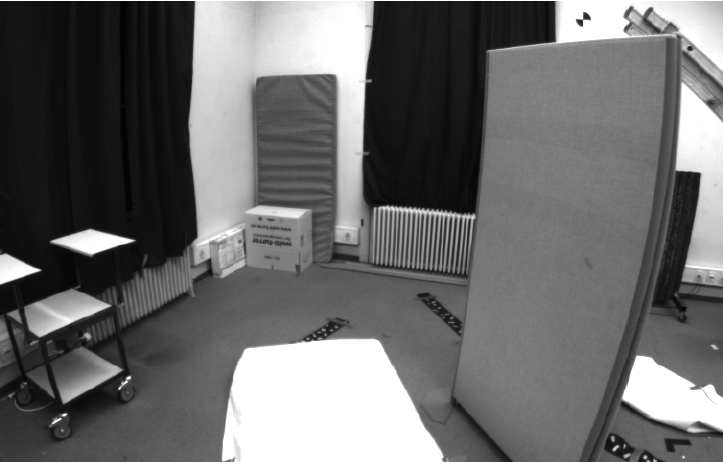
\includegraphics[width=1\linewidth]{imgs/SM2a.png}\\
    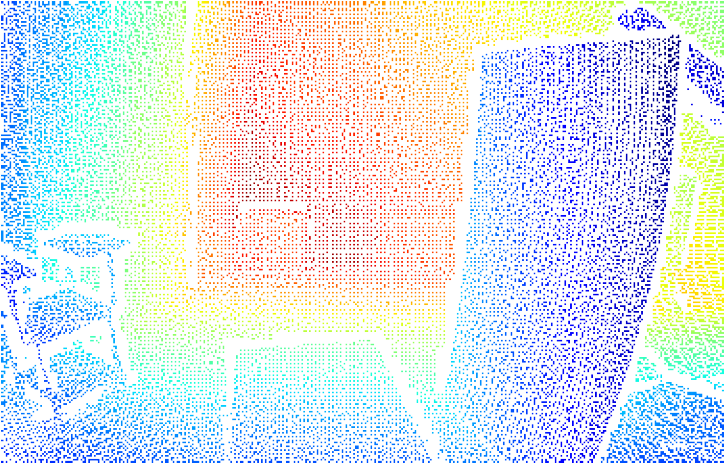
\includegraphics[width=1\linewidth]{imgs/SM2b.png}
  \caption*{Figure SM2. 生成的EuRoC数据集的深度图}
  
\end{figure}
\subsection*{A.6. YouTube8M IDs of used for training}
1ofm 2Ffk 2Gc7 2hdG 4Kdy 4gbW 70eK 77cq 7We1 8Eff 8W2O 8bfg 9q4L A8cd AHdn Ai8q B8fJ BfeT C23C C4be CP6A EOdA Gu4d IdeB Ixfs Kndm L1fF M28T M92S NSbx NSfl NT57 Q33E Qu62 U4eP UCeG VRdE W0ch WU6A WWdu WY2M XUeS YLcc YkfI ZacY aW8r bRbL d79L d9bU eEei ePaw iOdz iXev j42G j97W k7fi kxe2 lIbd lWeZ mw3B nLd8 olfE qQ8k qS6J sFb2 si9H uofG yPeZ zger

YouTube8M网站\footnote{\url{research.google.com/youtube8m/}}提供了将它们映射为YouTube ID的说明。每秒从每个视频中采样两个连续的帧。

\subsection*{A.7. EuRoC数据集的内参变换}
EuRoC集中的cam0的内参为:
\begin{equation*}
  \begin{bmatrix}
    458.654&0&367.215\\
    0&457.296&248.375\\
    0&0&1
  \end{bmatrix}
\end{equation*}
图像宽度和高度为(752,480), 径向失真系数为-0.28340811和0.07395907,高阶系数较小。在实验中,我们首先将图像中心裁剪到(704,448)。这既不会改变焦距,也不会改变失真系数,并且将x0和y0分别更改为343.215、232.375。接下来,我们将图像调整为(384,256),将所有与x相关的参数乘以384/704,将所有与y相关的参数乘以256/448。结果在表5的最后一列中。

\subsection*{A.8.里程计}
关于KITTI序列10的扩充如图SM3,表SM4和SM5所示。
\begin{figure}[htbp]
  \centering
    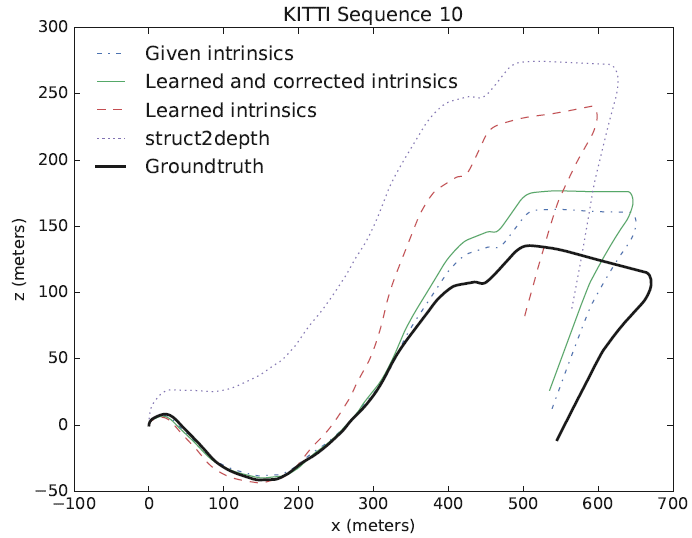
\includegraphics[width=0.9\linewidth]{imgs/SM3.png}\\
  \caption*{Figure SM3. 序列10的轨迹可视化}
  
\end{figure}

\begin{table}
  \centering
  \begin{tabular}{|c|c|c|}
  \hline
  Method&Seq. 09&Seq. 10\\
  \hline
  Zhou [47]            &0:021 ± 0:017& 0:020 ± 0:015\\
  Mahjourian [24]      &0:013 ± 0:010& 0:012 ± 0:011\\
  GeoNet [44]          &0:012 ± 0:007& 0:012 ± 0:009\\
  Godard [13]          &0:023 ± 0:013& 0:018 ± 0:014\\
  Struct2depth [6]     &0:011 ± 0:006& 0:011 ± 0:010\\
  \hline
  Ours, with intrinsics:&&\\
  Given                &0:009 ±0:015& 0.008 ±0:011\\
  Learned              &0.012 ±0:016& 0.010 ±0:010\\
  Learned \& corrected &0.010 ±0:016& 0:007 ±0:009\\
  \hline
  \end{tabular}
  \caption*{Table SM4. 扩展了主文件中的表6。}
\end{table}

\begin{table}
  \centering
  \begin{tabular}{|c|c|c|c|c|}
    \hline
     &\multicolumn{2}{c|}{Seq. 09} & \multicolumn{2}{c|}{Seq. 10} \\
    \hline
    Method & $t_{rel}$ & $r_{rel}$ & $t_{rel}$ & $r_{rel}$ \\
    \hline
    Zhou [47] a la [46] &17.8  &6.78 &37.9 &17.8\\
    Zhou [47] a la [31] &21.63 &3.57 &20.5 &10.9\\
    Zhan [46]           &11.9  &3.60 &12.6 &3.43\\
    Struct2depth [6]    &10.2  &2.64 &29.0 &4.28\\
    \hline
    Ours, with intrinsics:&&&&\\
    Given &3.18& 0.586& 5.38 &1.03\\
    Learned &7.47& 0.960& 13.2 &3.09\\
    Learned \& corrected &2.70& 0.462& 6.87& 1.36\\
    \hline
    \end{tabular}
  \caption*{Table SM5. 扩展了主文件中的表6。}
\end{table}

\begin{figure*}[htbp]
  \centering
    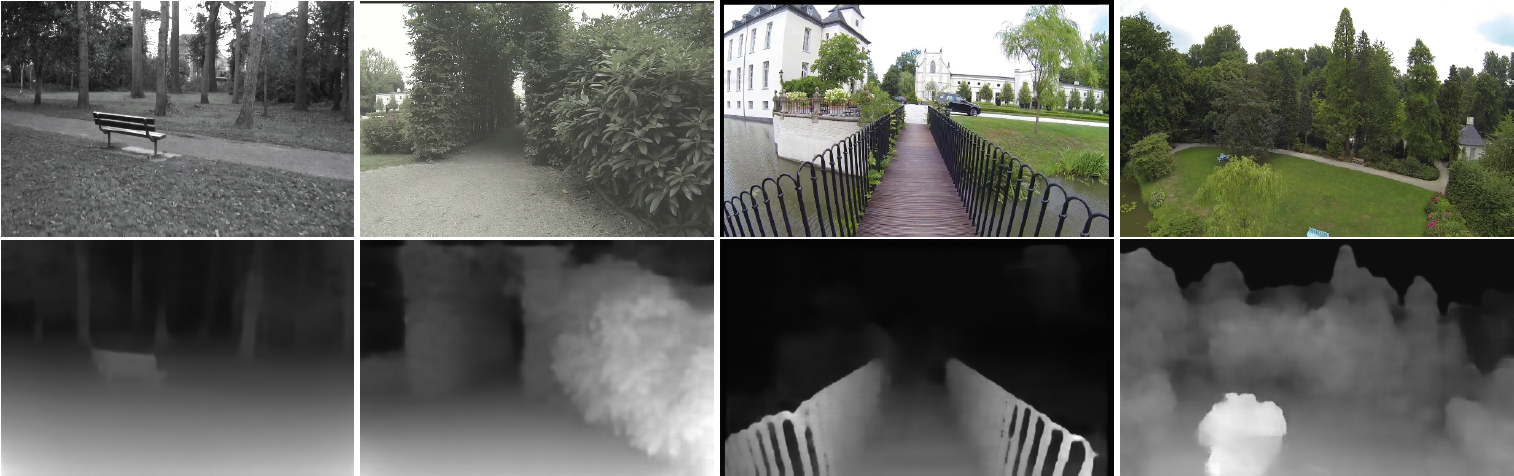
\includegraphics[width=0.9\linewidth]{imgs/SM1a.png}\\
    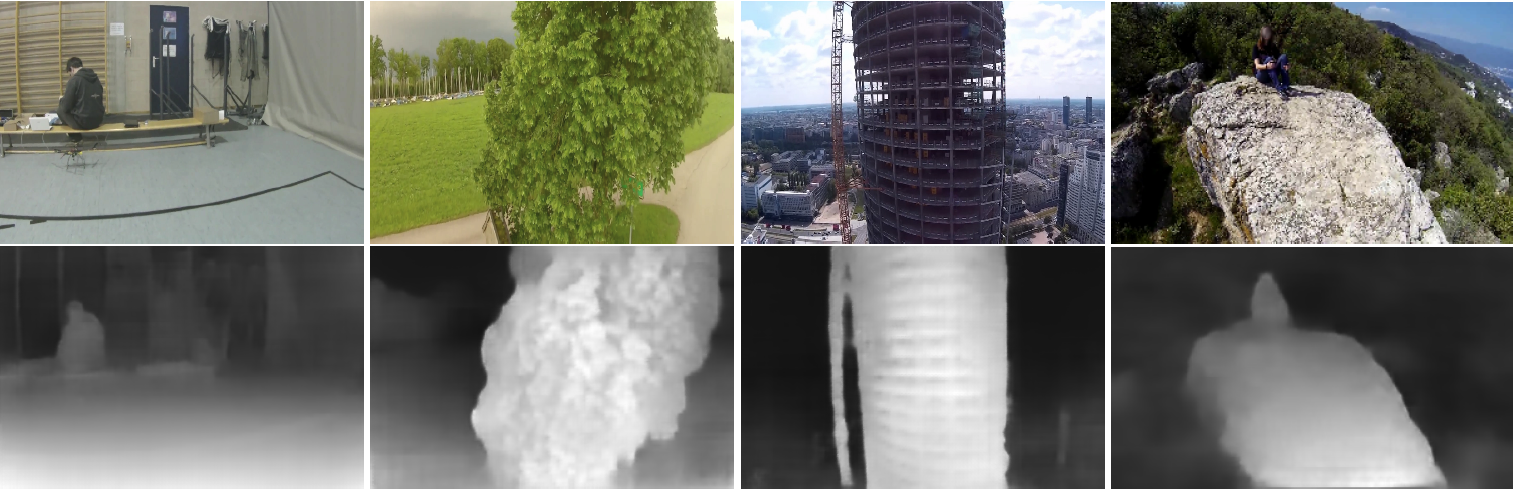
\includegraphics[width=0.9\linewidth]{imgs/SM1b.png}\\
    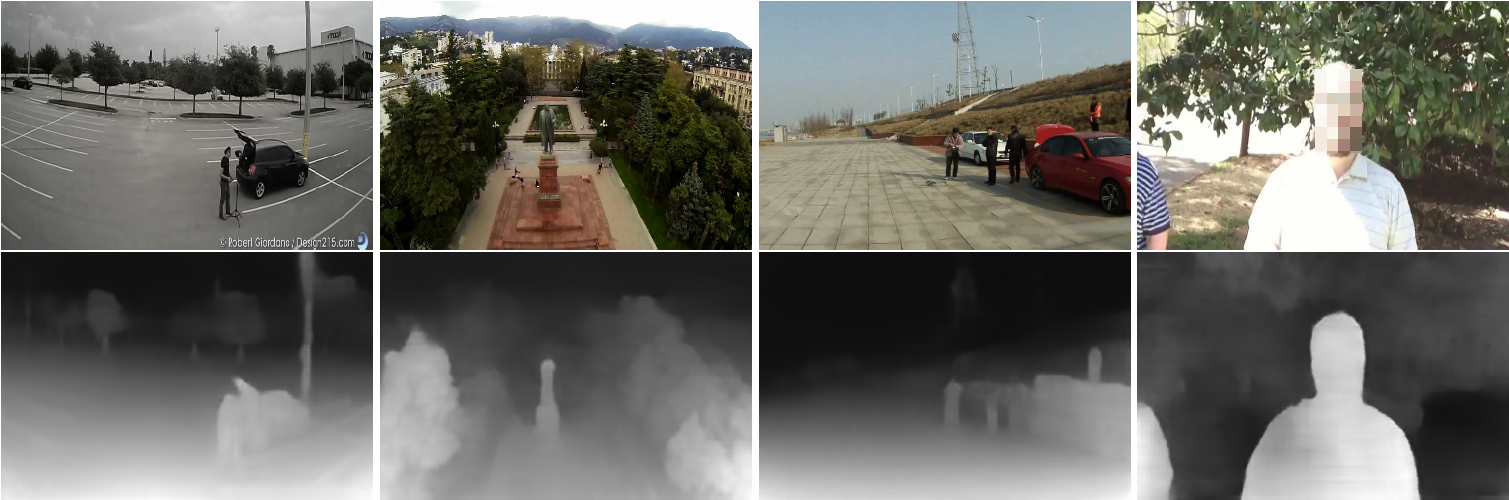
\includegraphics[width=0.9\linewidth]{imgs/SM1c.png}\\
  \caption*{Figure SM1. YouTube8M的实验结果}
\end{figure*}
% Can use something like this to put references on a page
% by themselves when using endfloat and the captionsoff option.
\ifCLASSOPTIONcaptionsoff
  \newpage
\fi

\cleardoublepage
% %% 参考文献
% \bibliographystyle{unsrt}
% \bibliography{ref}
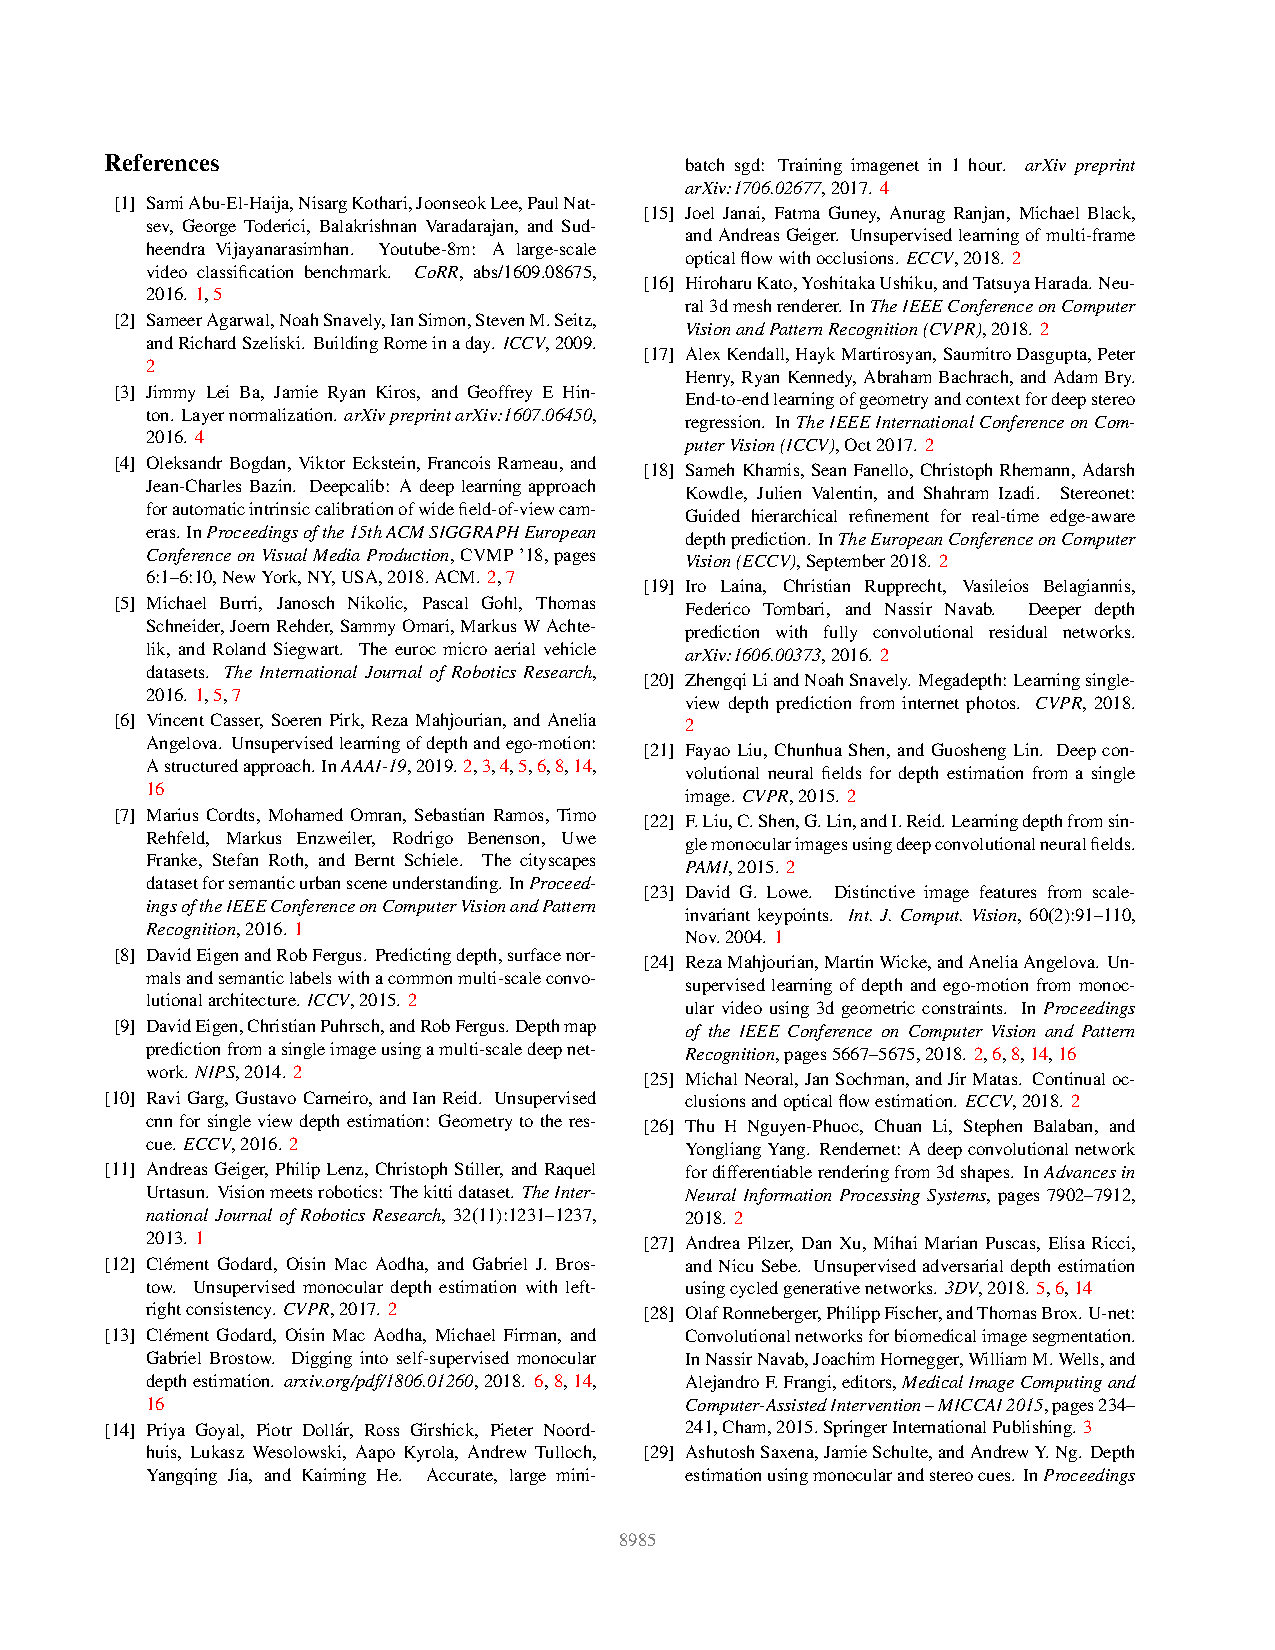
\includepdf[pages={1,2}]{ref.pdf}
\newpage
%%作者介绍
\begin{IEEEbiography}[{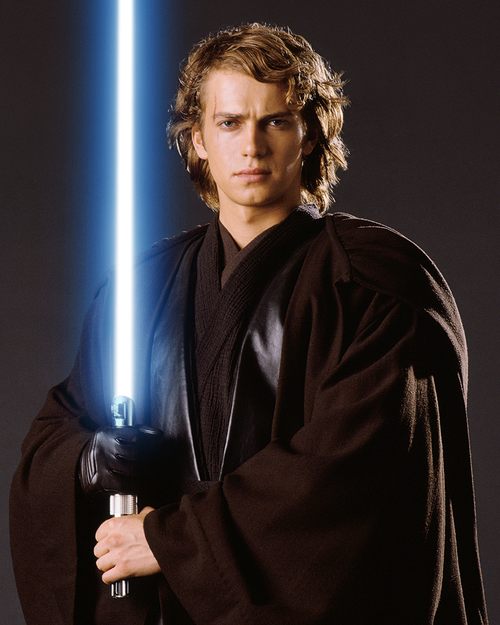
\includegraphics[width=1in,height=1.25in,clip,keepaspectratio]{imgs/Anakin_Skywalker.png}}]{Anakin Skywalker}
  Anakin Skywalker, a Force-sensitive human male, was a Jedi Knight of the Galactic Republic, a hero of the Clone Wars, and the Chosen One of the Force. During the reign of the Galactic Empire, he was known as Darth Vader, Sith Lord and apprentice to Emperor Darth Sidious. Skywalker was born in 41 BBY, forty-one years before the Battle of Yavin, on the planet Tatooine in the Outer Rim Territories of the galaxy. 
%%带照片
\end{IEEEbiography}
% if you will not have a photo at all:
\begin{IEEEbiography}[{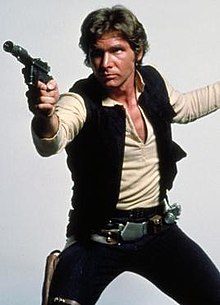
\includegraphics[width=1in,height=1.25in,clip,keepaspectratio]{imgs/Han_Solo.jpg}}]{Han Solo}
  Han Solo is a fictional character in the Star Wars franchise, who is a pilot from the planet Corellia. In the original film trilogy, Han is the captain of the Millennium Falcon, along with his Wookiee co-pilot Chewbacca, whereby both pilots became involved in the Rebel Alliance's struggle against the Galactic Empire. During the course of the Star Wars narrative, Han becomes a chief figure in the Alliance and the love interest of Princess Leia. In the sequel trilogy, Han is Leia's husband and the father of fallen Jedi, Kylo Ren.
%%不带照片
\end{IEEEbiography}
% insert where needed to balance the two columns on the last page with
% biographies
%\newpage
\begin{IEEEbiographynophoto}{R2-D2}
  R2-D2, or Artoo-Detoo, is a fictional robot character in the Star Wars franchise created by George Lucas. A small astromech droid, R2-D2 is a major character and appears in nine out of the ten Star Wars films to date. Throughout the course of the films, R2 is a friend to C-3PO, Padmé Amidala, Anakin Skywalker, Leia Organa, Luke Skywalker, and Obi-Wan Kenobi in various points in the saga.
\end{IEEEbiographynophoto}

%%文档结束
\end{document}


